\documentclass{sig-alternate-05-2015}
\usepackage{subscript}
\usepackage{tikz}
\usepackage{hyperref}
\usepackage{graphicx}
\usepackage{algorithm}
\usepackage{algpseudocode}
\usepackage{varwidth}
\usepackage{booktabs}
%\usepackage{algorithmicx}
\usepackage{amsmath}
%\usepackage[lined,boxed,longend,ruled]{algorithm2e}
\newcommand\mycommfont[1]{\footnotesize\ttfamily\textcolor{blue}{#1}}

%\AlgoDontDisplayBlockMarkers\SetAlgoNoEnd\SetAlgoNoLine%
\graphicspath{ {./imgs/} }

\begin{document}
\pagenumbering{arabic}
\title{Topic-zoomer: a URL categorization system}

\numberofauthors{2}
\author{
    \alignauthor
    Luca Giacomelli\\
           \affaddr{DISI\,-\,University of Trento}\\
           \affaddr{Student id: 179954}\\
           \email{luca.giacomelli-2@studenti.unitn.it}
    \alignauthor
    Pierfrancesco Ardino\\
           \affaddr{DISI\,-\,University of Trento}\\
           \affaddr{Student id: 189159}\\
           \email{pierfrancesco.ardino@studenti.unitn.it}
    }
\maketitle


\begin{abstract}
Smartphones and tablets pervade our lives on a daily basis and people use them in most curious ways.\\
The key idea behind this work is to take advantage of the traffic they generate while they are connected to the Internet, extracting \emph{topics} from what people search on the web with their mobile devices. This use case provides also the geographical coordinates of the users based on the telephone cell they are connected to.\\
For the purpose of this work the approximate location of the cell is enough, even though it implicitly defines a limit on the precision while selecting an area inside a map.\\
This paper presents Topic-zoomer, a URL categorization system.
\end{abstract}


\printccsdesc
\keywords{Data mining, URL categorization, topic extraction, geolocalized URLs, Latent Dirichlet Allocation}


\section{Introduction}
Nowadays extracting topics from a text is a very common goal in data mining and the problem of categorizing URLs is highly connected to it.\\
Generally speaking, the main purpose is to find out the topics of a set of documents. Applying this concept to a more specific problem, Topic-zoomer is able to find the topics of a dataset based on the documents' geographical location.\\
Starting from a geotagged dataset, the tool is able to restrict its space domain only to pages which are inside a certain area.
In this way, it can discover the topics of the various regions.\\
This work can be employed in many different fields. For example, it can be useful for public institutions such as municipalities; they could understand the citizens' needs in order to improve the functionality of the city's facilities and their territory coverage.\\
However, the main problem of a real-life usage of this kind of analysis can be the data source. Internet Service Providers (ISPs) can easily extract and provide geotagged URLs based on the HTTP requests passing through their routers. Furthermore, the anonymity of the users generating such traffic must be preserved.\\
This kind of problems is a challenge for traditional programming paradigms, since the amount of data can be huge and it may also involve streaming  processing.


\section{Related work}
URL categorization is a task that many people and companies are addressing in the last few years, pushing even to the categorization of the whole World Wide Web. Some of the companies involved in this kind of analysis are Cyren\footnote{\url{http://www.cyren.com/url-category-check.html}} and BrightCloud\footnote{\url{https://www.brightcloud.com/tools/change-request-url-categorization.php}}. Moreover, a huge number of academic researches have been published and also some patents\footnote{\url{https://www.google.com/patents/US8078625}} have been filed on the subject. However, the specific case of geotagged URLs has not raised so much interest neither in the academic nor in the developer communities.\\
Furthermore, when approaching problems related to Big Data or Data Mining, the challenge is to deal with huge amounts of data that cannot fit in a single machine or use smart solution to avoid useless computation. This implies that merely sequential solutions are not admitted, since they can be costly in terms of time. Instead it can be possible to use computations already done with the aim of reducing the amount of time needed for a run and at the same time trying to not losing accuracy on the results.
\begin{figure*}[t]
  \center{\includegraphics[width=0.55\textwidth]{solution.png}}
  \caption{The schema representing the overall solution.}
  \label{solution}
\end{figure*}
\section{Problem definition}
The task Topic-zoomer aims to solve can be better described starting from its \emph{input} and \emph{output} data.\\
The \emph{input} is a CSV file containing rows of the following form:
\begin{equation}\label{dataset}
    <latitude,\,longitude,\,\{url0\,|url1\,|...\,\}\,>
\end{equation}
The URLs are analyzed in order to identify the topics that are represented as a vector of words that very often appear together.\\
Let \emph{A} be an algorithm to compute such topics (eg. TF/IDF, frequent itemset or LDA), the algorithm \emph{L} gives as a result the topics of the dataset in general.\\
\emph{L} also allows the user to restrict the search in the dataset using the following parameters:
\begin{itemize}
    \item \emph{A}: the map area identified by top-left and bottom-right corners. This is the region of interest for retrieving the topics.
    \item \emph{S}: the size of the grid to be created inside the area \emph{A} (ie. the square side length).
    \item \emph{k}: the number of topics to search inside each square of the grid.
\end{itemize}
In this way \emph{A} is divided into squares of size $S \times S$ and the \emph{k} topics are identified inside each square.

For this tool \emph{A} is not directly given as input. In fact, the top-left and bottom-right corners are computed from the dataset taking the top-left and and bottom-right corners of the dataset. Also the number of \emph{k} is fixed to 3.
\section{Solution}
This section describes in details all the steps needed to realize this tool, from the initial web page download to the data analysis done with python. The order by which they are presented reflects the one that was followed during the experiments. Furthermore, Figure \ref{solution} represents the architecture of the overall solution.


\subsection{Data collection and preprocessing}\label{preprocessing}
The first task was to transform an initial dataset with the form shown in \ref{dataset} into another one of the form
\begin{equation}\label{datasetClean}
    <latitude,\,longitude,\,page\_text\,>
\end{equation}
A \emph{crawler} has been developed in order to follow the links in the dataset and download the web pages linked to them. This may seem a trivial operation at a first glance, but it is not really true. In fact, the initial dataset contained a lot of URLs pointing to images, videos, configuration files for mobile phones applications and many other elements that are far from being a text web page. To retrieve only sensible information, the crawler rejects all the requests not containing \emph{text/html} in the responses' header. This is the one which is usually populated by a web server when a client visits one of its pages. Last but not least, the crawler has been parallelized between multiple processes to minimize the download time. Multiple processes are preferred to multiple threads because Python, the language used to develop the crawler, is known to be subject to the Global Interpreter Lock\cite{gil} (GIL).\\
Finally, after this crawling phase, a new CSV file containing rows as described in \ref{datasetClean} is generated.
\subsection{Algorithm selection}\label{algorithmSelection}
After downloading the web pages, the dataset has to be cleaned.\\
Among all the ways to extract topic such as TF-IDF or a simple N{\"a}ive word count, the \emph{Latent Dirichlet Allocation}\cite{lda} (LDA) algorithm was chosen as \emph{L} to find the topics of the dataset in general. LDA is a generative and probabilistic model for collections of discrete data such as text corpora. It is a Bayesian hierarchical model, where each topic is modeled over an underlying set of topic probabilities. LDA is a good candidate when choosing between different methods to classify text. From a higher perspective LDA can be seen as a clustering technique, whose goal is to divide the document corpora given as input into \emph{k} clusters, which are the topics to be retrieved from the text.
In order to compute LDA, \textit{tokenized pages} are first of all used to create an \textit{id-term dictionary}, which is then used to compute a \textit{document-term matrix}. Then the LDA model is computed using \texttt{
ldamodel} from the \texttt{gensim} module. This Python module allows LDA model estimation from a training corpus. The model can also be updated with new documents in order to support online training. This function will be used later in one of the two recomputation methods developed for this tools.

\begin{algorithm*}[!t]
    \caption{Sequential topic computation}\label{alg1}
    \begin{varwidth}[h]{\textwidth}
	\begin{algorithmic}[1]
	\Procedure{sequential\_computation}{size, dataset}

        \State $dataset \gets read(dataset)$ \Comment{Load dataset}

        \State $oldModel\gets read(oldModel)$ \Comment{Load old dataset}
        \If{(size \% oldModel.size == 0 \&\& size!=oldModel.size)} \Comment{Check for recomputation}

        	\State $base,height$ = $calculate\_New\_Size(size,oldSize)$ \Comment{Calculate the new dimensions of the grid}
            \For{oldCorpus in oldModel.corpus}

            	\State $corpus[b][h] \gets update\_corpus(oldCorpus)$ \Comment{update corpus for each new square}

            \EndFor
            \If{($recType==1$)}
            \State $model \gets ldaModelUpdate(numTopics, NumWords,corpus,oldModel.dictionary)$\Comment{Recompute using ldaModelUpdate}
            \EndIf
            \If{($recType==2$)}
            \State $model \gets topicMerging(oldModel,corpus[b[h])$\Comment{Recompute merging the most relevant topics of each previously computated block}
            \EndIf

        \ElsIf{size!=oldModel.size}
        	\State $base \gets round(dataset.base / size)$\Comment{Calculate base of inner grid}
            \State $height \gets round(dataset.height / size)$\Comment{Calculate height of inner grid}
            \State $clean\_dataset,dictionary  \gets create\_dictionary(dataset)$ \Comment{Clean and tokenize dataset}
        	\For{clean\_page in clean\_dataset}
            	\State $b,h \gets getCoordinates(clean\_page)$ \Comment{Assign each text to the correct block of the $b \times h$ inner grid}
            	\State $text[b][h]\gets clean\_page$

            \EndFor
        	\For{b in base;h in height}


            	\State $corpus[b][h] \gets create\_Corpus(text[b][h],dictionary)$\Comment{Create dictionary and corpus for the ldamodel}
                \If{($corpus[b][h]!=empty$)}
                \State $model[b][h] \gets ldaModel(numTopics, NumWords,corpus[b][h],dictionary)$\Comment{Calculate the LDA model for each block}
                \EndIf
            \EndFor

        \EndIf
     \If{size!=oldModel.size}
     \If{($recomputation!=0$)}
     \State $save(model)$\Comment{Save model for reuse}
     \EndIf
     \State $printToCsv(model)$\Comment{Save results in a csv file}
    \EndIf
\EndProcedure
\end{algorithmic}
\end{varwidth}
\end{algorithm*}

\subsection{Process overview}
\label{overview}
The process of finding the most important topics for each area $S \times S$ after the crawling phase is composed as follows:
\begin{enumerate}
    \item \label{params} Provide Topic-zoomer with the parameters, \emph{S}, the location of the dataset and \emph{recType}, which is the kind of recomputation to be used (0 for no computation, 1 for using \texttt{ldaUpdate} and 2 for using merging technique).
    \item \label{load} Load the dataset (in CSV format) generated by the pre-processing phase described in Section \ref{preprocessing}.
	\item \label{corners} compute the top-left and the bottom-right corners from the dataset.
        \item \label{init} Create squares of dimension $S \times S$ (ie. compute the inner grid) using \emph{S} and the two corners computed in \ref{corners}.
    \item \label{checkS} Check if the new \emph{S} is a multiple of the old \emph{S} saved from previous computations. Remember that information of a computation are saved only if \emph{recType} is different from 0. If the new \emph{S} is a multiple of the old \emph{S} it means that it is possible to use the recomputation method defined by \emph{recType} (see Section \ref{avoidingRecomputation} for a more detailed explanation). If the new \emph{S} is a multiple of the old \emph{S} then the process skips directly to point \ref{save}. If the new S is equal to the old S the software terminates its execution.
    \item \label{remove} For page in the dataset remove punctuation and stopwords\cite{mmd} for the language of interest\footnote{In this specific case, Italian and English stopwords are removed due to the source of the dataset used for the experiments.} in order not to consider the most common short function words.
    \item \label{dictDataset} Create the \textit{id-term dictionary} from the whole cleaned dataset.
	\item \label{assign} Assign each pages to the respective square in the grid.
    \item \label{convert} Create a corpus for each square in the grid. This step is fundamental, as each page of the square has to be converted into  a \textit{word-term matrix}.
    \item \label{train} Train the LDA model of each square with the proper \emph{k} parameter and chosing between the \emph{single-core} or \emph{multi-core} implementation.
    \item \label{partial} Save results for future recomputation if \emph{recType} is different from 0.
    \item \label{save} Save the results in a csv file.
\end{enumerate}

%\begin{figure*}
%  \center{\includegraphics[width=0.8\textwidth]{spark_pipeline.png}}
%  \caption{All the steps of the Spark pipeline represented in detail.}
%  \label{spark_pipeline}
%\end{figure*}
All this steps will be explained in detail in the following sections.
%Steps \ref{load}, \ref{params}, \ref{init} and \ref{filter} are shown in Algorithm \ref{alg1} and Algorithm \ref{alg2}; step \ref{check} is described in Algorithm \ref{alg4}; steps \ref{remove}, \ref{convert}, \ref{train}, \ref{partial} and \ref{save} are defined in Algorithm \ref{alg3}.\\

\section{Implementation}\label{implementation}
In this section will be explained how this version of topic-zoomer was implemented.
This project was written in Python using mainly functions from Gensim Library. Other python packages that were used are NLTK (Natural Language Tool Kit) and Stop words, that simply contains a list of stop words in different languages.
\subsection{Pseudocode}

Algorithm \ref{alg1} shows the pseudocode of the project.
As stated in section \ref{overview}, there are four main parts: dataset pre-processing, the avoid-recomputation, computation and printing. Now each part will be explained in detail.
\begin{algorithm*}[t]
\caption{Create Dictionary}\label{cleanText}
\begin{algorithmic}[1]
\Procedure{create\_dictionary}{$dataset$}
	\State global\_text[], global\_dictionary[]\Comment{Create local variables}
    \For{page in dataset}
	\State text = toLowerCase(page.text)\Comment{convert upper case to lower case}
    \State text = regexpFilter(text, [a-zA-Z]+)\Comment{keep only words with at least a letter}
    \State text = tokenize(text)\Comment{Tokenize the document}
    \State text = removeStopWords(text)\Comment{Remove stop words}
   \State global\_text.append(page.x,page.y,text)\Comment{Save each entry with its coordinates}
   \State global\_dictionary.append(text)
    \EndFor
     \State dictionary = dictionary(global\_dictionary) \Comment{turn our tokenized dataset into a id <-> term dictionary}
    \State $return$ dictionary,global\_text   \Comment{return the dictionary of the whole dataset and the cleaned text for each entry}
\EndProcedure
\end{algorithmic}
\end{algorithm*}
\subsection{Pre-processing}
The first thing to do after reading the dataset is to make it usable. \newline
Since the goal is to find relevant topics in every block of size $s \times s$, the first step is to divide the dataset into blocks.
Figure \ref{blocks} shows how the total area(in red) is divided in blocks. In mathematical terms, if $size$ is the size of the block, $base$ is the base of the dataset and $height$ the height, then the inner grid will have dimension equal to $(base/size) \times (height/size)$, with both divisions rounded up to the nearest integer value.
\begin{figure}[h]
  \center{\includegraphics[width=0.25\textwidth]{blocks.jpg}}
  \caption{How the total area is divided in blocks}
  \label{blocks}
\end{figure}
The second part of this pre-processing regards the text documents of the dataset.
The dataset is cleaned using the $create\_dictionary()$ function, showed in algorithm \ref{cleanText}.\\
The $create\_dictionary()$ function starts with creating two variables, one for storing each entry of the dataset after it has been cleaned and one for storing all the text and creating the dictionary for the dataset. \\
Then each entry of the dataset is cleaned in the following way:
\begin{enumerate}
\item Convert the the text into lowercase characters.
\item Use a regular expression filter so only words are kept.
\item The text is tokenized, that means it becomes a structure of n tokens, each of them is a word.
\item Stop words are removed. Stop words are extremely common words that do not have any meaning for this purpose. In this function are removed italian and english stop words.
\item The cleaned text is stored with its coordinates, so in the future will be possible to assign it to its correct block. It is also stored in another variable, in order to create the dictionary of the dataset.
\end{enumerate}
After all the dataset is cleaned, a dictionary is created, that means that at each different token is assigned an id.\newline
The $create\_dictionary()$ function returns both the dictionary and the text.
The final step is assigning each cleaned text to its correct block. The $create\_dictionary()$ function returns the cleaned text in the form $<x\_coordinate>;<y\_coordinate>; <cleaned\_text>$. So the task consists in iterating and, after reading the coordinates of each text, appending the text to the correct block.
The final result will be a dictionary for the whole dataset and a $b\times h$ matrix with all the text.

\subsection{Computation}\label{cmpt}
The computation is done using the ldaModel function from the Gensim Library.\\
\begin{center}
$gensim.models.ldamulticore.LdaMulticore(
num_{topics}=topics_{no}, corpus, id2word=dictionary,workers = cpu_{cores-1},  passes=50)$
\end{center}
This function needs the previously calculated dictionary and a corpus, and returns a model with $num_{topics}$ topics.
For calculating the corpus the function $create\_corpus()$ was used. This function receives a dictionary and a tokenized text as input and returns a document-term matrix. In other words, using the dictionary and the tokenized list it returns a matrix where on one axis there are id index of the dictionary, on the other there are the tokens. Then they are counted and each cell represents the number of times each term has appeared.\\
In this project the number of topics is fixed at three, with three words for each one. This is because with more words or more topics the model it is not accurate and the results are not meaningful.\\
The number of passes indicates the Maximum number of iterations allowed to LDA algorithm for convergence. It is set to 50 because it is a good compromise between performance and  accuracy.
The multicore version was used because it has better performance than the single core version. The number of workers(threads that the ldaModel function will use), as depicted in the ldaModel documentation, is the number of physical cores minus 1. This means that if the cpu has more than two cores then the multicore version will be used otherwise it uses the single core version.
\subsection{Printing}\label{printing}
The last thing to do is printing the results.\\
The solution chosen for dislaying the outcome is a csv file.
In each row are written the coordinates of the block and three topics. It is structured in this way:
\begin{center}
< Top-Left corner >; < Bottom-Right corner >; < Topic with id 1 >; < Topic with id 2 >;< Topic with id 3 >
\end{center}
If a block is empty it is not printed.
After printing the software terminates its execution.

\subsection{Avoid-recomputation}\label{avoidingRecomputation}
These kind of tools in order to be usable needs not only to be accurate, but they have to perform well
also with respect to time and memory usage. \\ A tool that performs well in term of accuracy but needs an high amount of memory could be really expensive and one company could prefer less expensive tools, thus it is necessary to find a good compromise between performances and costs. \\ Use previous computations to quickly compute the topics for each of the new cells is a key point for this project and in general for these tools to be usable. As said before, two different recomputation methods have been developed and implemented for this project. Both are based on cell rescaling and merging of the cells in order to provide the zoom out feature. \\ It was decided to use the following simplification: resizing can only be done when the new size of the cell is a multiple of the old size of a cell. For example if the cell size of the previous computation was 2 and the new size is 3 then it is not possible to use recomputation and so a new computation will be done, otherwise the cell are rescaled and merged avoiding useless computation.
\begin{figure}[h]
  \center{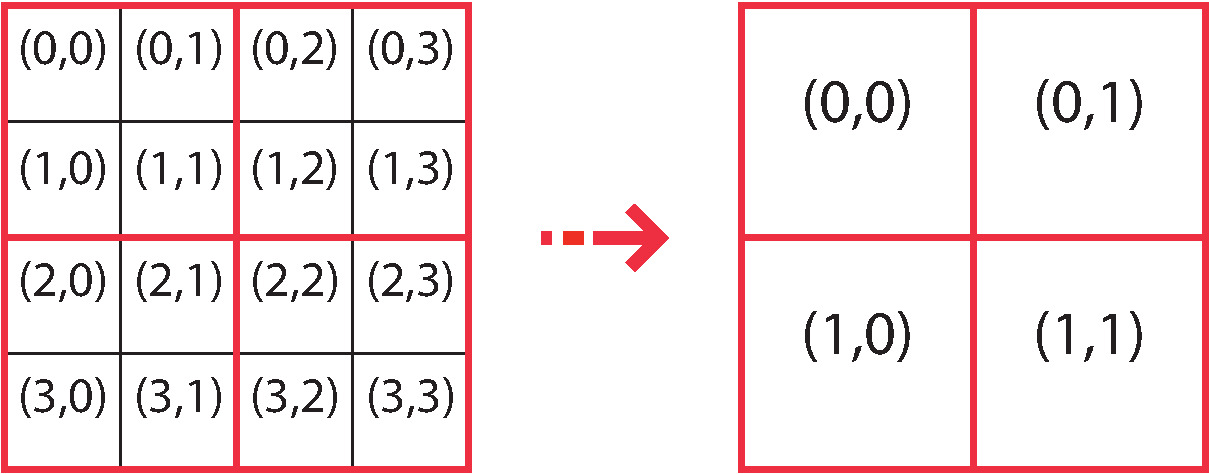
\includegraphics[width=0.45\textwidth]{resize.pdf}}
  \caption{An example of cell rescaling.}
  \label{resizeImg}
\end{figure}
\newline
For instance, figure \ref{resizeImg} shows the rescaling for a 4x4 map to a 2x2 map.
\subsubsection{Recomputation with \textit{ldaUpdate}}
The first recomputation method implements the \textit{ldaUpdate} function that updates an already computed model with new document. Taking as example the grid in Figure \ref{resizeImg}, at the beginning the ldaModel is computed for each cell in the grid and saved in a stable storage for future computations. The idea is to reuse and update one of the models. Cells (0,0), (0,1), (1,0), (1,1) of the grid on the left will compose the (0,0) cell of the 2x2 grid, so the model computed for the cell (0,0) can be used and updated with the corpus of the remaining cells. In general one of the cells that will compose the new cell is used as base model, while the corpus of the others will be used to update it. Algorithm \ref{rec1} shows the operation performed for the recomputation.
\begin{algorithm*}[h]
\caption{Recomputation with \textit{ldaUpdate}}\label{rec1}
\begin{algorithmic}[1]
\Procedure{recomputation\_ldaupdate}{$dataset$}
	\State to\_merge = newStep / oldStep,
    \State y = 0
    \State y\_old = 0
    \While {y\_old < height\_old}
    	\State x\_old = 0
    	\State x = 0
    	\While {x\_old < length\_old}
			\State corpus\_to\_merge = []
    		\For{i in range (0,to\_merge)}
    			\For{j in range (0,to\_merge)}
    				\If{not ldaModelMatrix[x][y] and corpus\_old[y\_old +i][x\_old + j]}
   						\State ldaModelMatrix[y][x] = ldaModelMatrix\_old[y\_old + i][x\_old + j] \Comment{Use an old ldaModel as base}
   					\Else
   						\State corpus\_to\_merge += corpus\_old[y\_old + i][x\_old + j] \Comment{Merge the corpus of the cells}
   					\EndIf
   				\EndFor
   			\EndFor
   			\If{ldaModelMatrix[y][x]}
   				\State ldaModelMatrix[y][x].update(corpus\_to\_merge) \Comment{Update the base model with the merged corpus}
   			\EndIf
   			\State x\_old += to\_merge
   			\State x +=1
   		\EndWhile
   		\State y\_old += to\_merge
   		\State y +=1
    \EndWhile
\EndProcedure
\end{algorithmic}
\end{algorithm*}

\subsubsection{Recomputation with topic merging}
The second recomputation method counts how many times the topics of the old cells appear in the new corpus, returning the most probable topics. Again, taking as example the grid in Figure \ref{resizeImg}, the  topics of cells (0,0), (0,1), (1,0), (1,1) of the grid on the left are inserted into an array, while the corpus of these cell will compose the corpus of cell (0,0) on the right grid. Then the \textit{topic\_update} function will compute how many times each topic of the array appears in the new corpus. Algorithm \ref{rec2} shows the operation performed for the recomputation.
\begin{algorithm*}[h]
\caption{Recomputation with \textit{topicMerging}}\label{rec2}
\begin{algorithmic}[1]
\Procedure{recomputation\_topicmerging}{$dataset$, $topics$}
	\State to\_merge = newStep / oldStep,
    \State y = 0
    \State y\_old = 0
    \While {y\_old < height\_old}
    	\State x\_old = 0
    	\State x = 0
        \State corpus\_to\_merge = []
    	\While {x\_old < length\_old}
			\State corpus\_to\_merge += corpus\_old[y\_old + i][x\_old + j]
    		\For{i in range (0,to\_merge)}
    			\For{j in range (0,to\_merge)}
   				\EndFor
   			\EndFor
   				\State ldaModelMatrix[y][x] = topic\_update(corpus\_to\_merge, dictionary, topics) \Comment{Compute the new topics}
   			\State x\_old += to\_merge
   			\State x +=1
   		\EndWhile
   		\State y\_old += to\_merge
   		\State y +=1
    \EndWhile
\EndProcedure
\Function{topic\_update}{$corpus$, $dictionary$, $topics$}
\State topic\_occ = \{\}
\For{ topic in topics}
	\For{page in corpus}
		\For{token in page}
			\If{dictionary[token[0]] == topic}
				\If{topic not in topic\_occ}
					\State topic\_occ[topic]=token[1]
				\Else
					\State	topic\_occ[topic] += token[1]
				\EndIf
			\EndIf
		\EndFor
	\EndFor
\EndFor
\State total\_topics = sum(v for k,v in topic\_occ.items())
\State \Return RankedAndSortedTopics(topic\_occ, total\_topics)

\EndFunction
\end{algorithmic}
\end{algorithm*}
\section{Results}\label{results}
The final step consists of measuring the overall performances.\newline
For doing so, this software was executed with squares of side equal to 4. Then with side equals to 8, using all the possible techniques (normal computation and the two types of recomputation). The table \ref{exectime} shows the execution time for each technique:\\
\begin{table}[h]
\centering
\caption{Execution time}
\label{exectime}
\begin{tabular}{@{}|l|l|l|@{}}
\toprule
Square's side & Computation technique  & Time   \\ \midrule
4             & Normal computation     & 4045 s \\ \midrule
8             & Normal computation     & 2662 s \\ \midrule
8             & "Merge" recomputation  & 11 s   \\ \midrule
8             & "LdaUpdate" recomputation & 640 s  \\ \bottomrule
\end{tabular}
\end{table}
Looking at this table it is easy to see that the proposed recomputation algorithms are faster than the normal algorithm.\\
After looking at the performance it is time to compare the quality of the results using the proposed algorithms.\\
From the quality point of view there were some problems related to the dataset (like broken links, links to pages with irrelevant or absent content etc.) but we can see that the results are coherent and the recomputation techniques give results that are meaningful using a faster computation. \\ Just for giving an insight, choosing a step equal to 8 the results related to the first square are \emph{diritti  rai  http ; type  itemid  x ; x  f  mm ;} and with the two recomputation techniques the following topics were obtained \emph{rai;diritti;type;} and \emph{f  mm  type ; x  dl  diritti ; test  page  d ;}.\\
In conclusion, this method does work but there is still room for further improvements like an adwanced crawler that filters all the pages retriving only meaningful information useful for this type of analysis.

\section{Conclusions and future work}
The algorithms implemented in this projects are three, as explained in sections \ref{cmpt} and \ref{avoidingRecomputation}.\\
The first is an implementation of the LDA and the other two are designed for avoiding recompuations in certain cases (when the new side is bigger and a multiple of the previous side). \\
The first recomputation method is based on the LDA update function of the GENSIM library, it basically merges the squares into a bigger one, avoiding the recomputation of the area given by the formula $ number\_of\_new\_squares \times area\_old\_squares $. This gives quite the same results of the LDA model.\\
The second recomputation method takes the probability for the most probable topics for each old square and averages them for finding the most probable new topics. Obviously this method is less reliable but really fast.\\
Section \ref{results} shows the performance of these algorithms. Unfortunately, due to the problems of some links of the dataset, an in depth analysis of the results from the quality and reliability point of view was not feasible but there is reason to believe that with a better dataset or crawler the aforementioned algorithms will work.\\
This project could be improved in many different ways, left as future works, like the implementation of a GUI for choosing in a user-friendly manner the square's area or an area different from a square. The possibility of chosing different areas will lead to new aprroaches for the avoiding recomputaion techniques, that will be more similar to the first recomputation method.\\
Another improvement will be the creation of a crawler designed for searching only on certain web pages related to the area of interest of the final user.\\
In conclusion it is possible to assert that this project is suitable for finding topics in areas divided in squares and a good starting point for user-defined areas, in both cases using geotagged URLs.\\





%\end{document}  % This is where a 'short' article might terminate
%
% The following two commands are all you need in the
% initial runs of your .tex file to
% produce the bibliography for the citations in your paper.

\bibliographystyle{abbrv}
\bibliography{biblio}% biblio.bib is the name of the Bibliography in this case

% You must have a proper ".bib" file
%  and remember to run:
% latex bibtex latex latex
% to resolve all references
%
% ACM needs 'a single self-contained file'!
%

\end{document}
